\chapter{循环流化床锅炉燃烧系统先进控制应用}
\label{chap:application}
在完成先进控制系统与DCS通讯及DCS组态后,接下来需要建立各回路的数学模型,并完成控制器参数的整定,以获得满意的控制效果。自衡对象选用一阶惯性纯滞后模型,非自衡对象选用积分纯滞后模型,模型参数采用离线数据进行辨识,控制器为阶梯式广义预测控制器,控制器参数在线整定。

\section{数据预处理}
\label{sec:pre_cal}
数据预处理包含数据校正和数据变换两部分。数据校正的目的主要是减少测量误差的影响,这里的测量误差分为过失误差和随机误差两种。数据变换的目的是减少不同数据单位差异的影响,以免降低模型的准确性和鲁棒性。

\subsection{数据校正}
过失误差的产生一般是由于仪表失灵或者记录错误。根据工业现场工艺要求的最大值和最小值,可以剔除一部分具有过失误差的数据。此外,还可以根据数据的统计规律,当某个数据点太过偏离平均值时,就可能具有过失误差。随机误差一般是由测量噪声和采样量化误差导致的。工业过程中,由于复杂多变的工艺环境及传感器本身的测量机理,测量值往往具有较大的随机误差。为了减小随机误差,多点滑动平均和一阶滤波是两种常用的方法。

$K$点滑动平均滤波取$K$步测量值的均值作为当前的测量值的滤波值,如式~\ref{equ:ma-filter}。多点滑动平均的幅频特性是低通的,其响应曲线与$\sin{x}/x$相似。这种滤适用于具有高频噪声的信号,但对偶然出现的脉冲性干扰的抑制作用较差。滑动平均滤波点数$K$的设置会对其性能有较大影响,在过程控制系统中一般根据测量点的特性选择。对于流量等回路噪声较大的回路,$K$可以取8-12;对于压力、液位等回路,$K$可以取4-8;对于温度等慢回路,$K$可以取1-4。
\begin{equation}
\label{equ:ma-filter}
{x'}_{i}=\frac{1}{K}\sum_{j=0}^{K-1}{x_{i-j}}
\end{equation}


一阶滤波式如式~\ref{equ:first_order_filter},$\alpha$为滤波系数。一阶滤波的幅频特性也是低通的,适用于缓慢变化的物理量,对周期性干扰有良好的抑制作用,但不能滤除高于1/2采样频率的噪声,且具有一定的相位延迟。$\alpha$一般取$[0.9,\,1]$
\begin{equation}
\label{equ:first_order_filter}
{{x}'_{i}}=\alpha {x_{i}} + (1-\alpha){{x'}_{i-1}}
\end{equation}

\subsection{数据变换}

由于本文中使用的是线性模型,而工业过程中的模型往往是非线性的,因此需要在工作点处作线性化处理。数据变换将系统的工作点迁移到0,这样避免了过程初始状态对后续状态的影响。工业环境中不同变量的变化范围差别很大,直接利用原始数据建立的模型参数过大或者过小,都会导致建模效果较差。将不同单位的数据缩放到同一范围,可以有效地改善建模的效果,增强算法的稳定性。

最典型的数据变换就是数据的归一化处理,即将数据统一映射到或者区间$[0,\,  1]$上。常用的归一化方法有z-score标准化和max-min标准化,此外还有log函数转换和atan函数转换。max-Min方法将将数据统一映射到,但当有新数据加入时,可能导致max或者min的变化,需要重新计算。对来自正态分布的样本,z-score标准化后的数据经过处理的数据符合标准正态分布,即均值为0,标准差为1。
\begin{align}
x'&=(x - \textrm{min})/(\textrm{max}- \textrm{min}) \\
x'&=(x - \mu)/{\sigma} \\
x'&={\log_{10}{x}}/{\log_{10}{\textrm{max}}}\\
x'&={2\arctan{x}}/{\pi}
\end{align}

\begin{figure}[!htb]
\centering
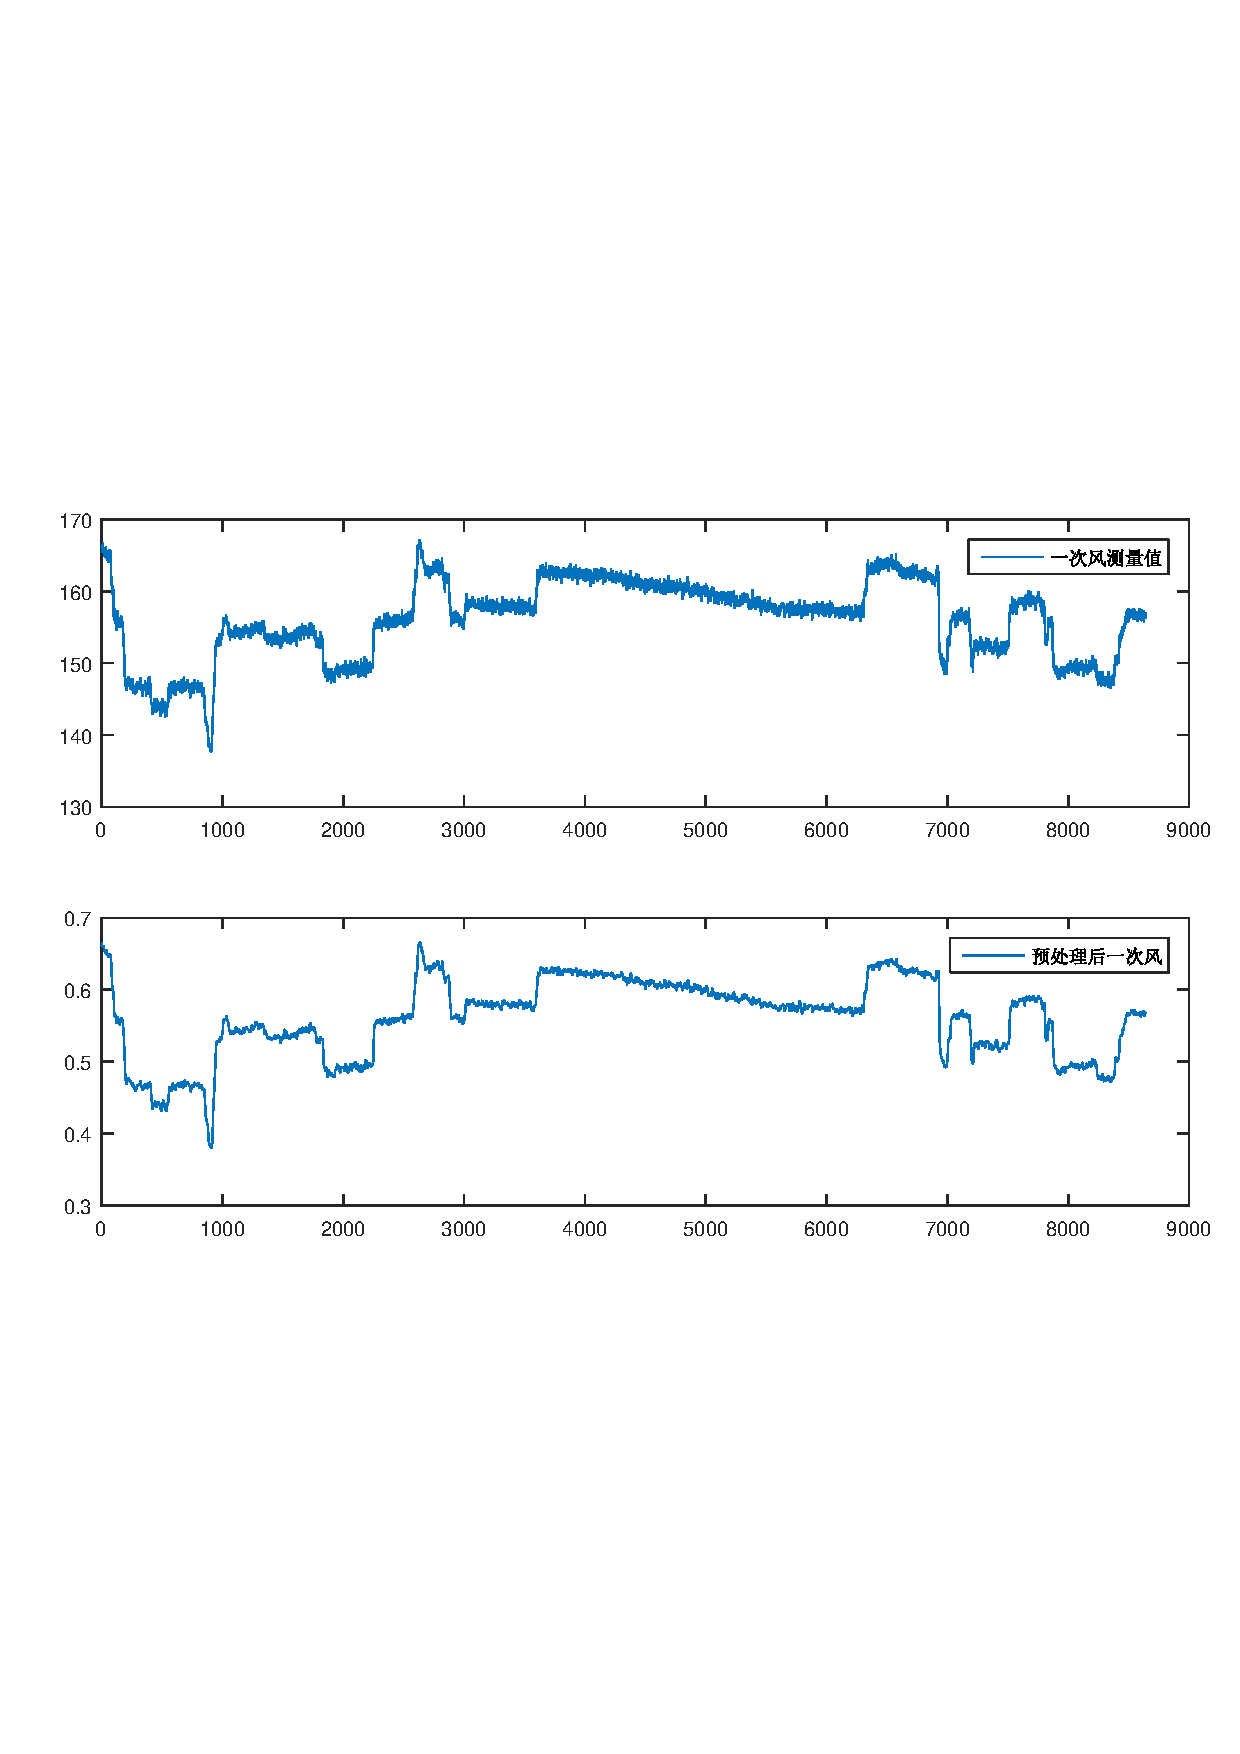
\includegraphics[width=13cm]{pre_cal}
\caption{一次风量数据预处理} \label{fig:pre_cal}
\end{figure}

以一次风量为例,采用五点滑动平均和Max-Min标准化对其进行数据预处理后的曲线如图~\ref{fig:pre_cal}~所示。这里的Max和Min分别采用一次风上限200和下限100,经预处理后数据被映射到$[0,\, 1]$,且包含的噪声明显减少。



\section{系统辨识}
\label{sec:mod_ide}

系统辨识是建立系统数学模型的一种方法。Ljung对辨识下定义为:“辨识有三个要素:数据、模型和准则。辨识就是按照一个准则在一组模型中选择一个与数据拟合得最好的模型”。大量的过程运行数据保存在工厂的数据库中,为系统辨识提供了基础。工业过程中大部分对象为自衡对象,可以采用一阶惯性纯滞后模型来描述,少部分非自衡对象可以用积分纯滞后模型描述。信息准则描述了模型与实际系统的接近程度,辨识算法与选用的信息准则是紧密相关的,几乎所有的辨识算法都是根据极大化或者极小化某个信息准则推导出来的\cite{陈霸东2011系统参数辨识的信息准则及算法}。

\subsection{辨识算法}
在选定模型结构和信息准则后,就可以利用经过预处理的数据辨识模型参数。经典的辨识信息准则主要有最小二乘准则、最小均方误差准则和极大似然准则,对应的辨识算法分别为最小二乘类算法、最小均方算法和极大似然法。其中,最小二乘类算法计算简单,对噪声的先验特性要求不高,是过程控制中常用的辨识算法。此外,辨识准则还包括非均方辨识准则和信息论辨识准则,前者适用于非高斯噪声环境,后者不仅适用于非线性非高斯情况下辨识信号处理,还适用于模型结构确定\cite{陈霸东2011系统参数辨识的信息准则及算法}。

1795年,Gauss(高斯)提出了最小二乘法的基本概念,并把其应用于天文计算中。最小二乘法的目标是样本辨识误差的平方和最小。由Guass-Markov(马尔可夫)定理,最小二乘法在随机误差项均值为零、方差恒定、互不相关等条件下,成为最优线性无偏估计\cite{montgomery2015introduction}。下面是最小二乘法的计算步骤。

假设系统由公式~\ref{equ:ls}~描述
\begin{equation}
\label{equ:ls}
y = \sum_{j=1}^{q}{\theta_{j}}{x_{j}}+\varepsilon
\end{equation}
其中$y$为系统输出,$x_{j}$为第$j$个系统输入。

如果有$n$组测量,可以转成矩阵形式,令$\bm{\theta} = {\begin{pmatrix} \theta_{1} & \theta_{2} &\cdots & \theta_{q} \end{pmatrix}}^{T}$为待估计量,系统的描述为 
\begin{equation}
\bm{Y} = \bm{X}\bm{\theta} + \bm{\varepsilon}
\end{equation}
其中$\bm{X} = \left[{\begin{array}{cccc}
x_{1}{(1)}  & x_{2}{(1)}&\cdots&x_{q}{(1)}\\
x_{1}{(2)}  & x_{2}{(2)}&\cdots&x_{q}{(2)}\\
\vdots & \vdots &\ddots  &\vdots\\
x_{1}{(n)}  & x_{2}{(n)}&\cdots&x_{q}{(n)}
\end{array}}\right]$

参照最小二乘准则的定义,给出式~\ref{equ:tar_identify}~所示的目标函数
\begin{equation}
\label{equ:tar_identify}
{S}(\bm{\theta})=\sum_{i=1}^{n}{\varepsilon_{i}^{2}}=(\bm{Y}-\bm{X}\bm{\theta})^{T}(\bm{Y}-\bm{X}\bm{\theta})
\end{equation}

令目标函数对$\bm{\theta}$的偏导数为0,得到如下式的待估计量:
\begin{equation}
{\bm{\theta}}=(\bm{X}^{T}\bm{X})^{-1}\bm{X}^{T}\bm{Y}
\end{equation}

最小二乘法要求系统的输入信号已知,但由于系统中输出相对输入有一定的纯滞后,对于某一特定输出序列,其输入序列实际上是未知的。因此,需要先确定系统的纯滞后时间,然后才能利用最小二乘法来辨识模型的参数。最常用的纯滞后时间确定方法为阶跃响应曲线法。但工业过程中某些对象不允许进行阶跃试验,而且测量的噪声问题使得滞后时间的确定存在一定的主观性。相关系数法可以较准确地从历史数据中计算出系统的滞后时间。对输入量$x_{i}$ 和输出量$y$ ,可以计算滞后$k$ 步的输入与输出之间的相关系数。使得相关系数绝对值最大的步数即为系统输出相对输出的滞后步数,滞后步数与采样时间之积为滞后时间。此外,还可以选择多段数据分别计算滞后时间,最后取中位数或者众数作为最终的滞后时间。
\begin{align}
\tau_{i} &= \underset{k}{\arg\max}|{\rho(\bm{X}_{i}^{(0)},\bm{Y}^{(k)})}|\times{T_{s}}\\
\rho(\bm{X},\bm{Y})&=\frac{E[(\bm{X}-\mu_{\bm{X}})(\bm{Y}-\mu_{\bm{Y}})]}{\sigma_{\bm{X}}\sigma_{\bm{Y}}}
\end{align}
其中$\bm{Y}^{(k)}$代表样本$\{y(k+1),\,y(k+2),\,y(k+3),\,\cdots,y(k+n)\}$,$\bm{X}_{i}^{0}$代表样本$\{x_{i}(1),\,x_{i}(2),\,x_{i}y(3),\,\cdots,x_{i}(n)\}$,$\tau_{i}$为第$i$个输入量相对$y$的滞后时间,$T_{s}$为数据采样时间。
 
\subsection{主汽压力回路参数辨识}
主汽压力回路广义控制对象的输入为给煤同操,输出为主汽压力。这是一个自衡对象,可以采用一阶惯性纯滞后模型,传递函数的形式如~\ref{equ:trans_func}。式中$K$反映了对象的静态特性,$T$反映了对象的动态特性,$\tau$反映了对象的输出相对于输入的滞后时间。
\begin{equation}
\label{equ:trans_func}
G(s) = \frac{K}{1+Ts}e^{-\tau{s}}
\end{equation}
 
由相关系数法确定为主汽压力与给煤同操器之间的滞后时间$\tau$后,即可利用最小二乘法辨识模型的增益$K$与惯性时间$T$,得到传递函数如式~\ref{equ:_gas_pre_tans_func}。
\begin{equation}
\label{equ:_gas_pre_tans_func}
G(s) = \frac{5.5}{1+180s}e^{-30{s}}
\end{equation}
主汽压力回路还有针对主汽流量的前馈环节。因此,还需辨识主汽流量为输入,主汽压力为输出的对象模型。由于前馈环节为静态前馈,该模型不需要特别准确,只需要辨识静态增益。
\subsection{床温回路参数辨识}
床温采用串级控制策略,应分别建立主、副回路的数学模型。主回路的广义控制对象为一次风风煤比-床温,副回路广义控制对象为一次风导叶开度-一次风量。回路的副回路模型可以根据历史运行数据得到,主回路模型需要在副回路投入自动控制后,根据新的数据进行参数辨识。主回路的传递函数如式~\ref{equ:_bed_tem_tans_func}~所示,一次风分AB两侧,这里给出A侧传递函数,如式~\ref{equ:_first_flow_tans_func}。
\begin{equation}
\label{equ:_bed_tem_tans_func}
G(s) = \frac{-5.5}{1+300s}e^{-120{s}} 
\end{equation}
\begin{equation}
\label{equ:_first_flow_tans_func}
G(s) = \frac{0.4}{1+20s}e^{-6{s}}
\end{equation}

 
\subsection{床层压差回路参数辨识}
床层压差回路的控制对象为冷渣器转速-床层压差,这是一个非自衡对象,其模型为
\begin{equation}
\label{equ:tans_func}
G(s) = \frac{K}{s}e^{-\tau{s}} = \frac{-0.4}{s}e^{-200{s}}
\end{equation}
 
同理,由于增加了针对给料量的前馈环节,还需辨识给料量为输入,床层压差为输出的对象模型,这也是一个非自衡对象,也只需辨识其增益$K$。


\section{各回路控制器参数整定及控制效果}
根据4.2节中模型辨识的结果,对先进控制器的参数进行整定。回路的整定顺序为床层压差回路、床温回路、主汽压力回路。床温回路实际上包含主回路和副回路,其整定顺序为副回路、主回路。

\subsection{控制器参数整定原则}

图~\ref{fig:gpc_tunning}~为先进控制软件的参数整定界面,当前界面为主汽压力回路的参数整定。其中操作变量和控制变量量程由现场工艺确定,模型增益、惯性时间、纯滞后等参数由~\ref{sec:mod_ide}~节系统辨识算法确定,需整定的参数包括控制周期、预测步长、控制步长、柔化因子、阶梯因子、控制上下限、增量上下限、前馈系数、滤波方式等。
\begin{figure}[!htb]
\centering
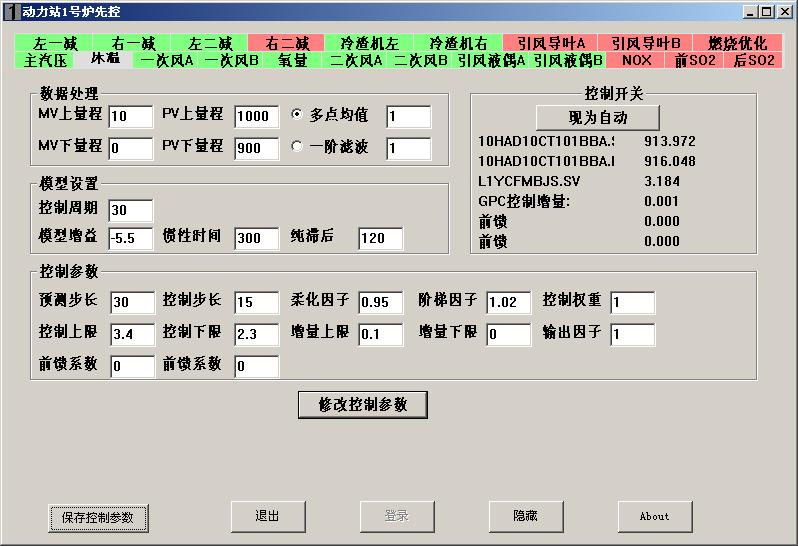
\includegraphics[width=13cm]{gpc_tunning}
\caption{先进控制系统参数整定界面} \label{fig:gpc_tunning}
\end{figure}

控制周期$T_{c}$既可以根据香农定理利用频率特性确定,也可以根据对象的特性结合工程经验选择。控制周期太大的话,控制作用会变慢;控制周期太小的话会增加控制系统的计算量,也可能导致系统不稳定。对于开环稳定对象,控制周期一般取为模型开环阶跃上升时间的$\textrm{1}/\textrm{10}$\,-\,$\textrm{1}/\textrm{4}$之间。
\begin{subequations}
\begin{align}
p &= \max{(10,\ t_{r}/T_{c})} \label{equ:steady1}\\
p &= t_{95}/T_{c} \label{equ:steady2}\\
p &= d_{\max}+t_{r}/\textrm{3.5}T_{c} \label{equ:with_dealy}
\end{align}
\end{subequations}

预测步长$p$的取值有很多方式。Clarke等指出对于大多数过程控制系统,预测步长取10是合适的\cite{clarke1987generalized}。对于开环稳定对象,也可以将预测步长与系统上升时间结合起来,如式~\ref{equ:steady1}~和~\ref{equ:steady2}~所示。对于具有纯滞后环节的回路,也有如式~\ref{equ:with_dealy}~的取法\cite{garriga2010model}。式中$t_{r}$为上升时间,$t_{95}$为上升至稳态值95$\,$$\,$\si{\percent}~所用时间,$d_{\max}$为系统最大纯滞后步数。

 
控制步长$p_{u}$是系统完成控制目标所需的步数。控制步长增大,允许系统在更多步完成控制目标,可以提高系统的鲁棒性,但系统的计算量也随之增加。在模型准确的情况下,可以取$p_{u}$为1或者控制对象的开环不稳定极点数。为了增强系统的鲁棒性,$p_{u}$可以取$p/\textrm{4}$。在系统工作点经常变化或者非线性较强导致模型失配的情况下,$p_{u}$可以取得更大。

控制权重$\lambda$影响控制器对控制量变化的容忍程度。控制权重越大,控制量的变化范围越小,系统鲁棒性越强,控制作用越慢\cite{1991Analysis}。在未对数据归一化的系统中,控制权重的取值与变量的单位相关。如果已经对数据进行了归一化处理,典型的控制权重在0.6到2之间。

柔化因子$\alpha$的取值范围为$[0,\ 1)$,这个参数保证了系统输出值经过比较平滑的轨迹达到期望输出。但当预测步长较大的时候,柔化因子可能会失效。柔化因子越大,系统控制速度越慢,被控量的轨迹也越平滑。Seborg等提出了基于期望系统闭环时间常数的柔化因子整定方法。

阶梯因子$\beta$是两个相邻控制量增量的比例,阶梯因子大于1时,第一步控制量较小,被控量变化较慢,系统鲁棒性强。阶梯因子小于1时,系统反应速度较快,但鲁棒性也会降低\cite{罗国娟2006阶梯式预测控制器的参数整定研究}。

控制上下限和控制量增量上下限与现场工艺有关,并没有一般性的设置方法,需要与现场的操作人员协商后设置。

前馈系数的由辨识出的模型决定。如图~\ref{fig:ff}~所示的前馈环节。前馈控制器的传递函数如式~\ref{equ:ff_trans_func}~所示。本文采用的静态前馈控制器只需满足稳态增益的要求,如式~\ref{equ:ff_static}~所示。
\begin{figure}[!htb]
\centering
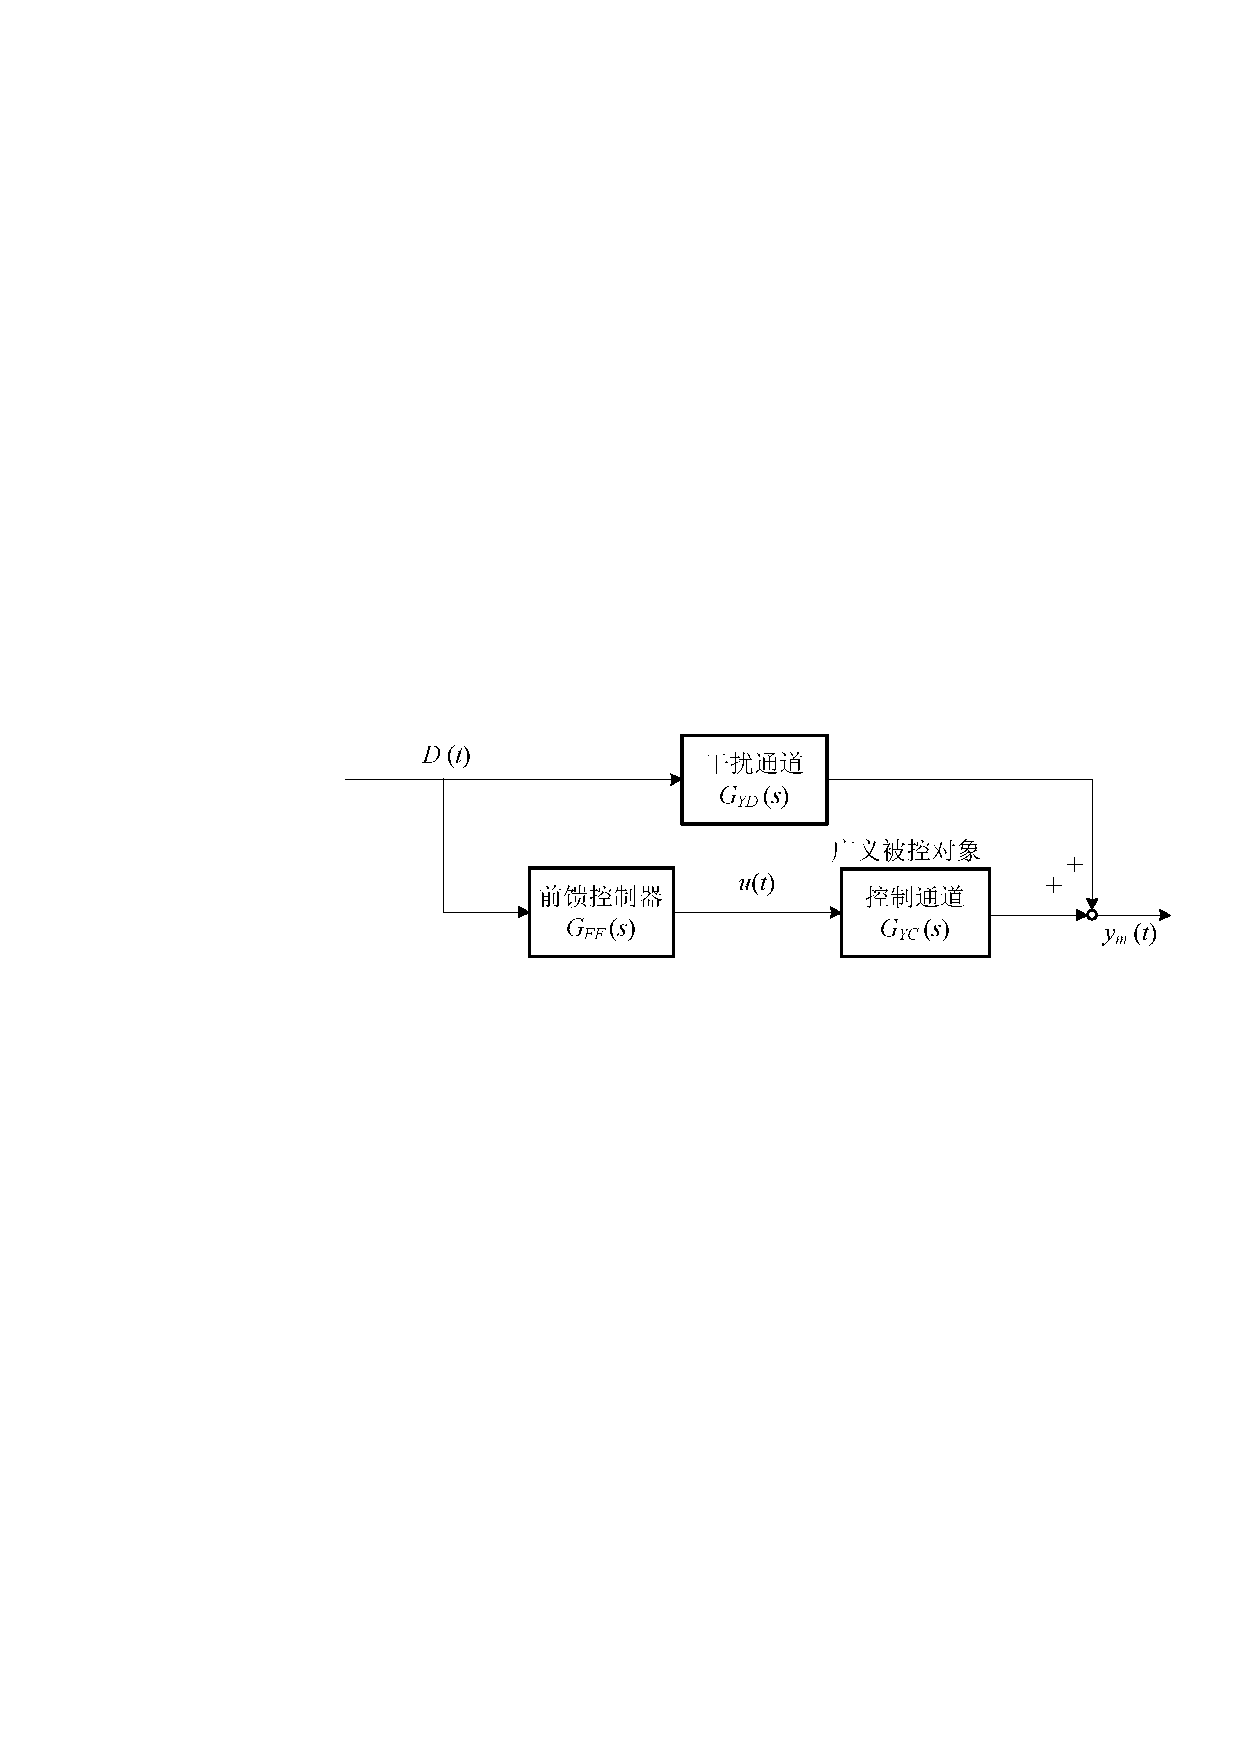
\includegraphics[width=13cm]{ff}
\caption{前馈控制} \label{fig:ff}
\end{figure}
\begin{equation}
\label{equ:ff_trans_func}
G_{FF}{(s)} = -\frac{G_{YD}{(s)}}{G_{YC}{(s)}}
\end{equation}
\begin{equation}
\label{equ:ff_static}
K_{FF} = -\frac{K_{YD}}{K_{YC}}
\end{equation}
 
滤波方式的选择有多点均值和一阶滤波两种,其设置方法见~\ref{sec:pre_cal}~节。

\begin{figure}[!htb]
\centering
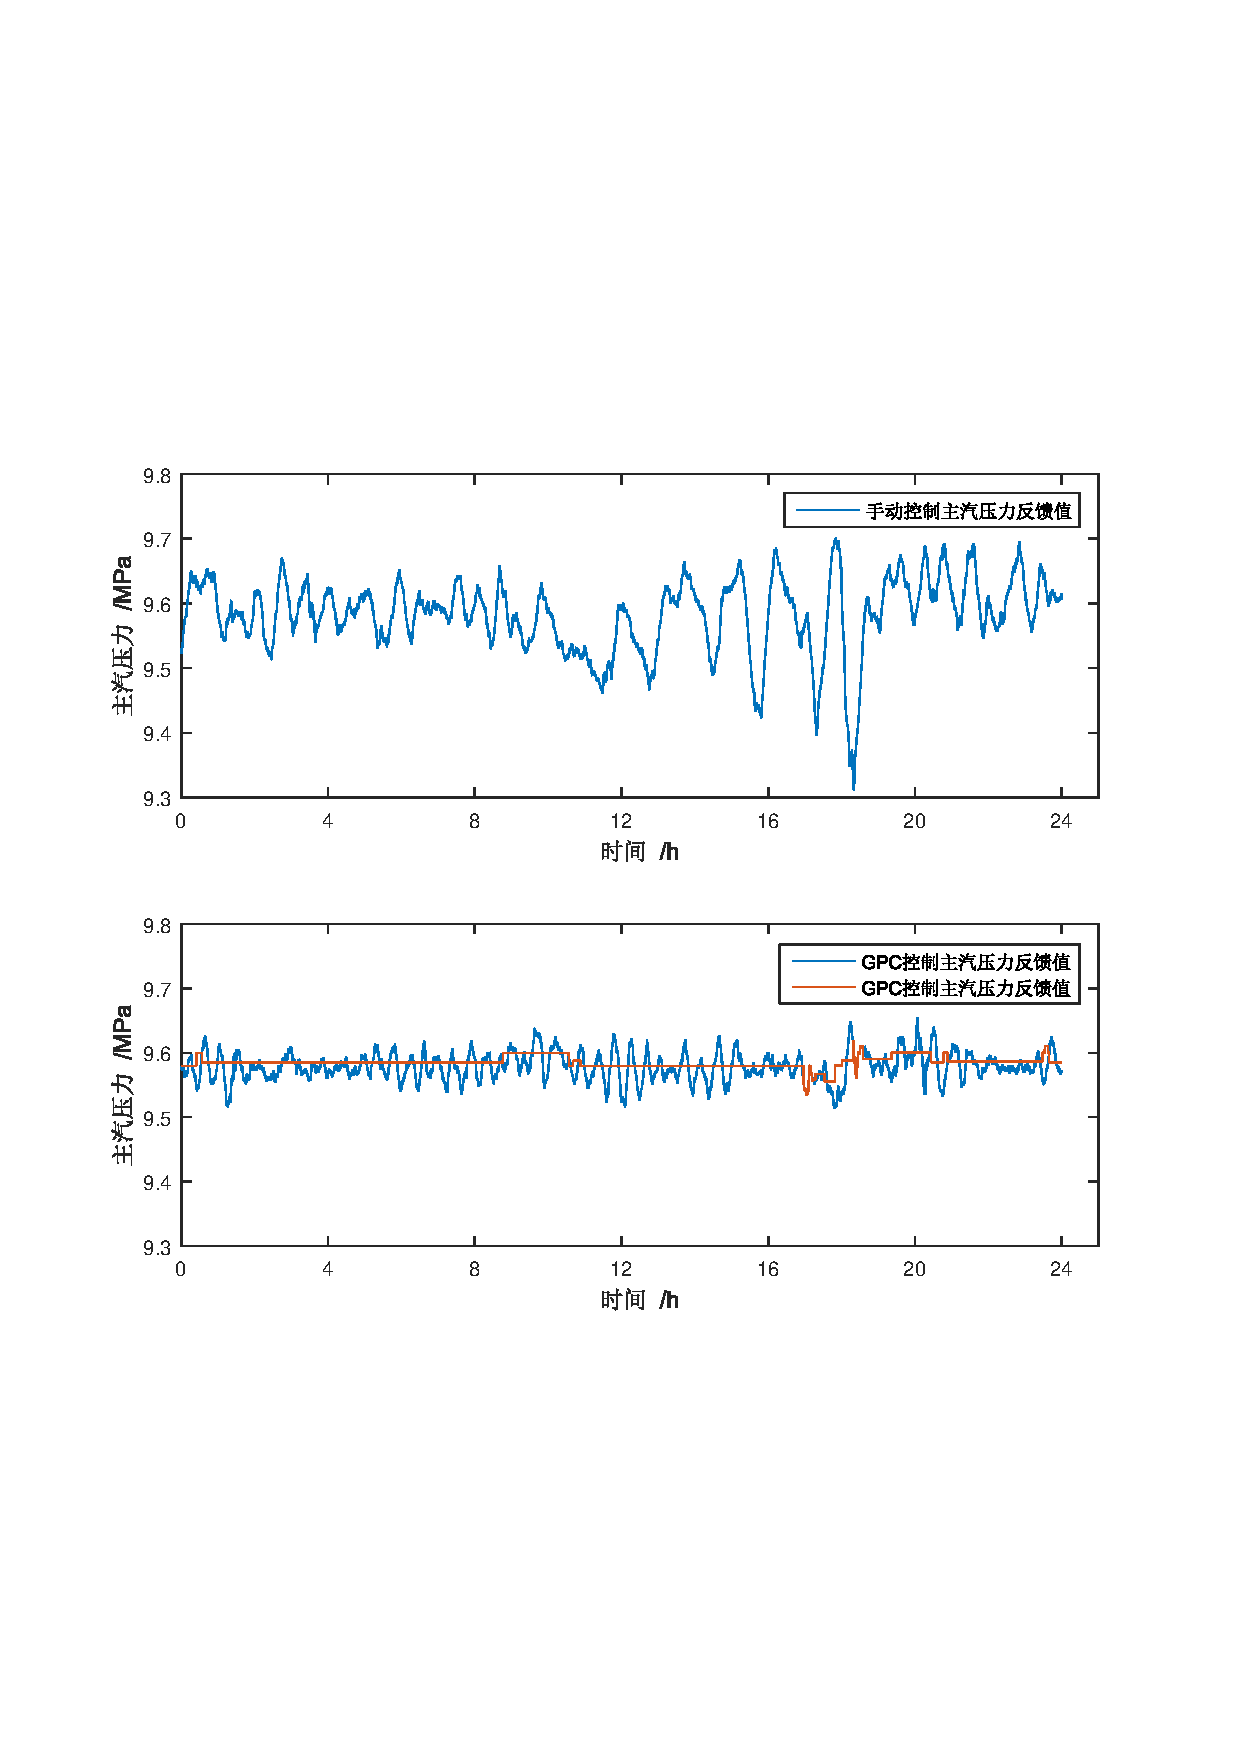
\includegraphics[width=13cm]{gas_pre_line_gpc}
\caption{主汽压力回路控制效果对比} \label{fig:gas_pre_line_gpc}
\end{figure}



\subsection{主汽压力回路控制效果}
图~\ref{fig:gas_pre_line_gpc}~对比了手动控制和先进控制的主蒸汽压力运行曲线。上侧为未投预测控制时的主蒸汽压力曲线,下侧为投入预测控制后主蒸汽压力运行曲线,均为24小时的曲线。手动控制时,锅炉的主汽压力波动幅度非常大,甚至从12时开始出现发散的趋势,严重危及下游生产设备的安全。投运GPC先进控制后,主蒸汽压力波动幅度明显减小,也能很好的跟踪设定值的变化。控制精度负荷平稳时$\pm$0.05$\,$$\,$\si{\mega\pascal},负荷波动较大时$\pm$0.07$\,$$\,$\si{\mega\pascal}。

\begin{figure}[!htb]
\centering
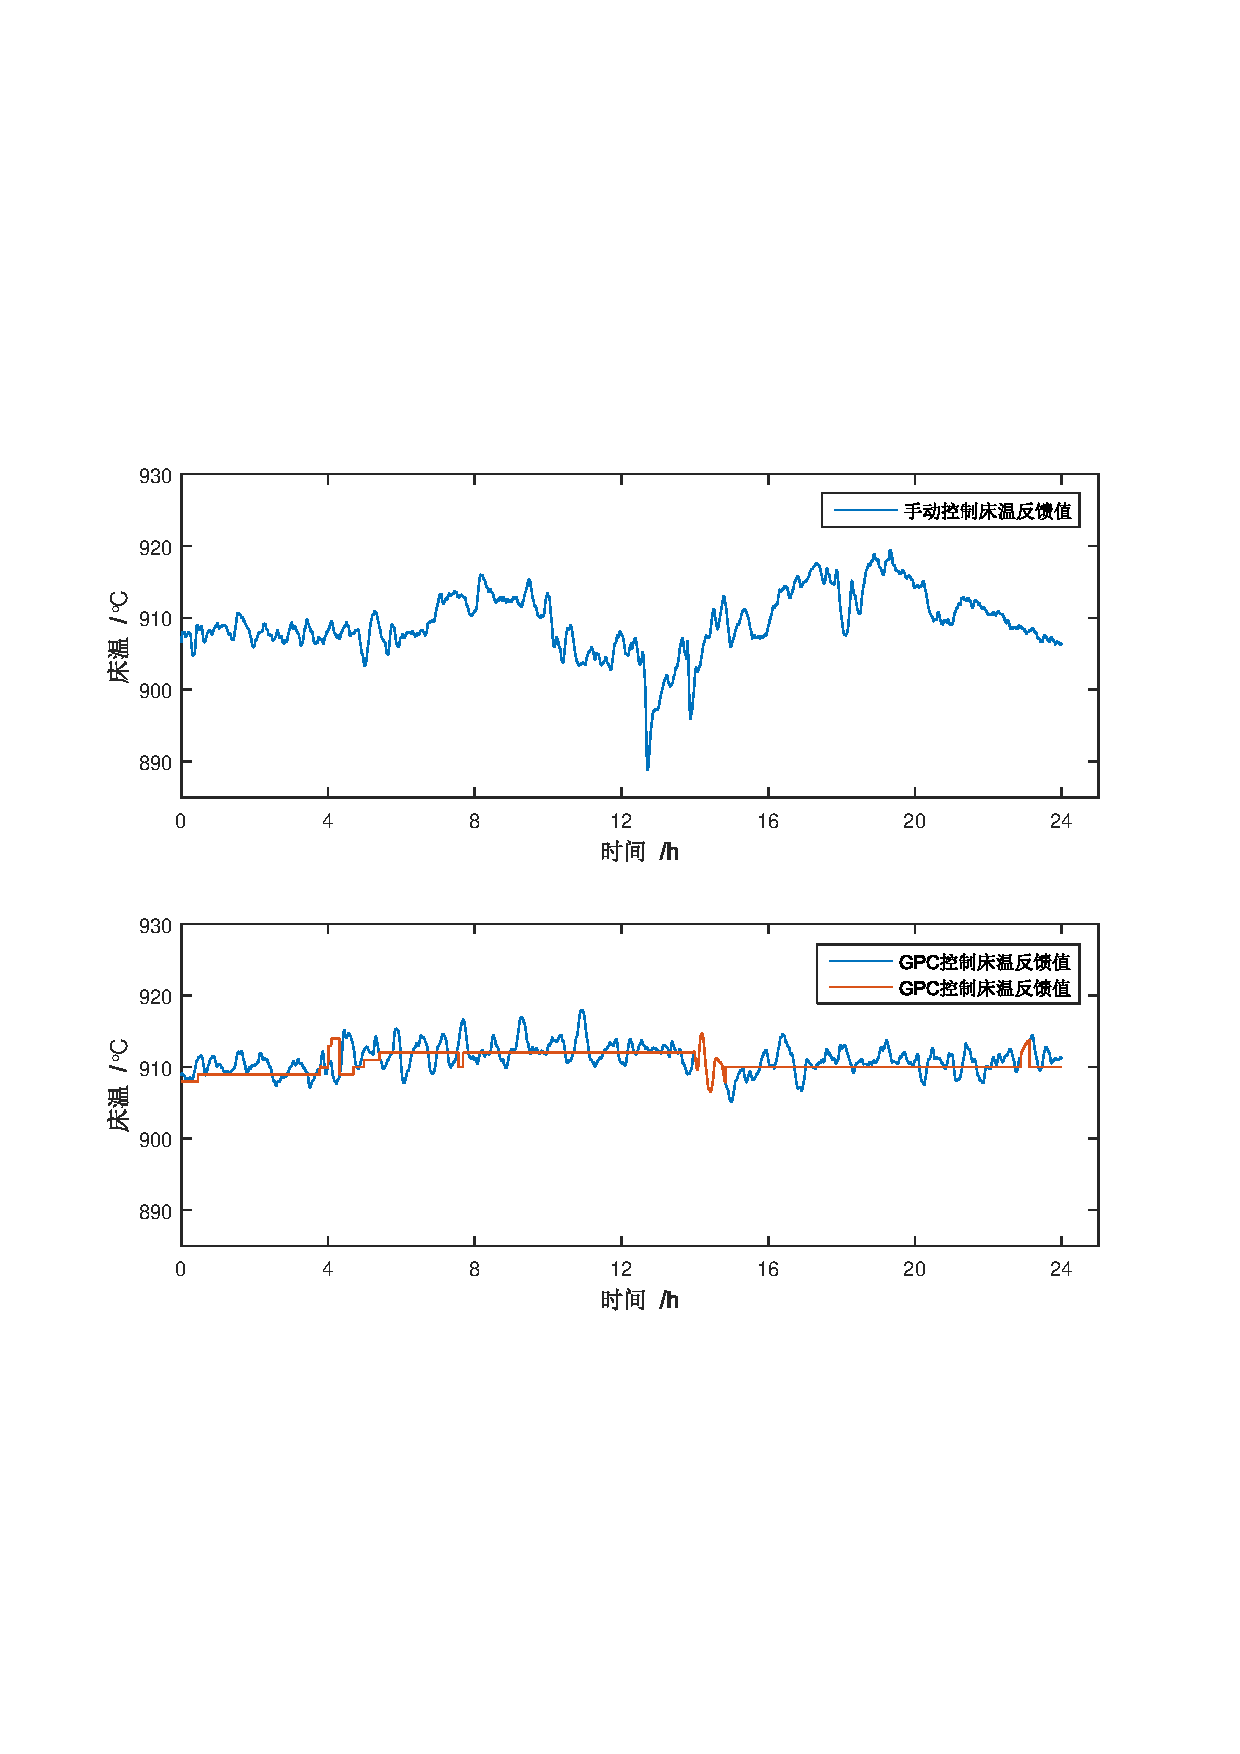
\includegraphics[width=13cm]{bed_tem_line_gpc}
\caption{床温回路控制效果对比} \label{fig:bed_tem_line_gpc}
\end{figure}
\subsection{床温回路控制效果}
图~\ref{fig:bed_tem_line_gpc}~对比手动控制和GPC先进控制的床温曲线。上侧为手动控制的床温曲线,下侧GPC控制的床温区曲线。在手动控制的时候,床温受锅炉负荷和给煤量影响,波动幅度很大。而投入先进控制后床温曲线的波动幅度明显降低,负荷变化不超过10$\,$\si{\percent},控制精度$\pm$3$\,$\si{\degreeCelsius},负荷变化较大时控制精度$\pm$5$\,$\si{\degreeCelsius},同时能很好的跟踪设定值调整。

\begin{figure}[!htb]
\centering
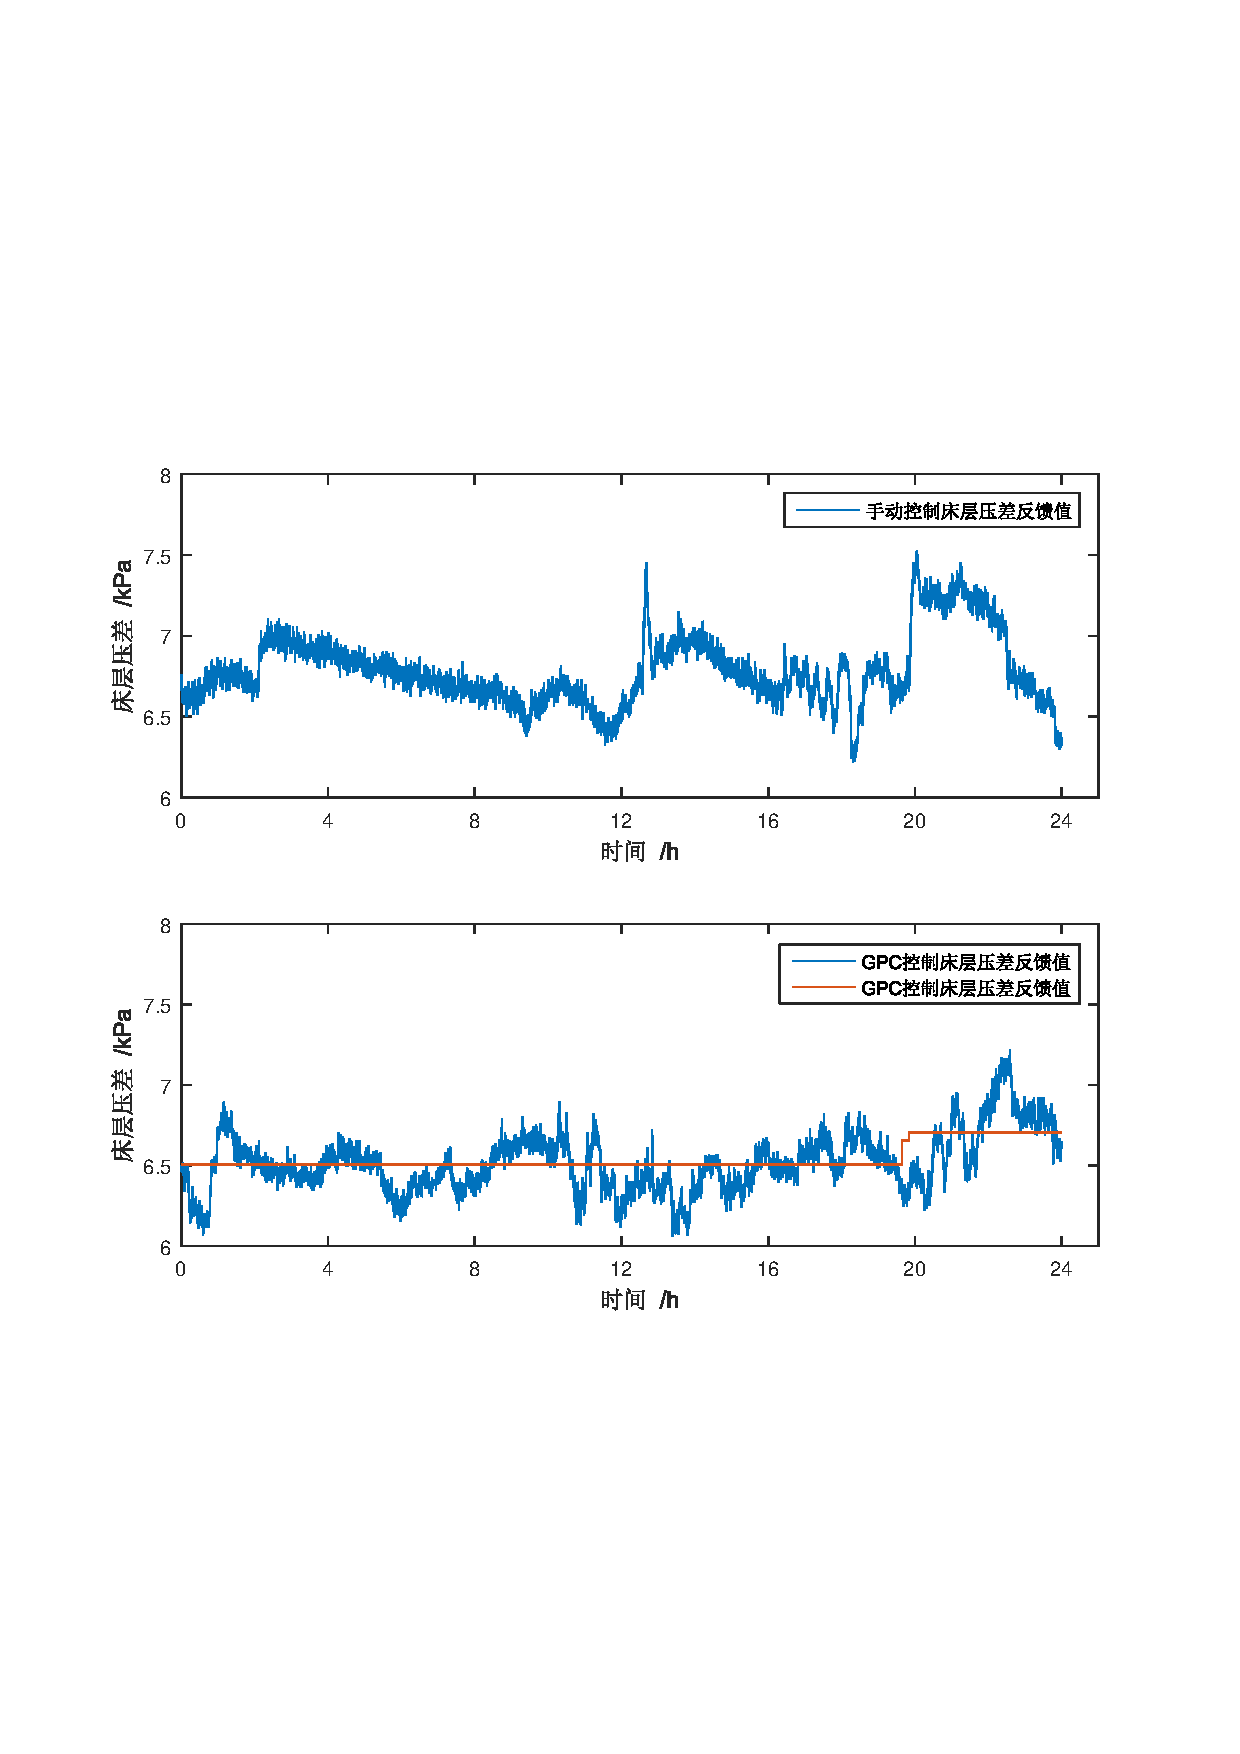
\includegraphics[width=13cm]{bed_pre_line_gpc}
\caption{床层压差回路控制效果对比} \label{fig:bed_pre_line_gpc}
\end{figure}
\subsection{床层压差回路控制效果}

图~\ref{fig:bed_pre_line_gpc}~为整日投入床层压差的对比曲线。上图为全天手动控制曲线,下图为GPC控制曲线。可以看到,手动控制时的随意性较大,床层压差时高时低,对燃烧有一定影响。投运GPC先进控制之后,床层压差始终在设定值范围波动,即使在设定值调整之后,也能比较快的跟踪设定值。由于这时候“床温—床层压差—一次风回路”已经投入自动,床层压差受一次风的影响较大,虽然控制精度显得不太高,但已经满足了现场的工艺要求。

另外,由于手动控制时床层压差控制不稳,为了使循环流化床的保持的正常流化状态,床层压差取的值较大,接近7.8$\,$\si{\kilo\pascal}。这会导致一次风机耗电量增加。投运先进控制后,床层压差设定值基本固定在6.5$\,$\si{\kilo\pascal},减少了一次风机耗电,提高了锅炉效率。


\subsection{先进控制效果总结}

最终先控系统达到的控制品质如表~\ref{tab:performance}。
\begingroup
\renewcommand*{\arraystretch}{1.67}
\begin{table}[!h]
\small
\caption[先进控制系统控制品质]{先进控制系统控制品质} 
\label{tab:performance}
\centering
\begin{tabular}{cccc}
\hline\hline
     &主汽压力  &   床温  &   床层压差\\
\hline
被控量偏差均值 &  -0.0067$\,$\si{\mega\pascal} &  0.604$\,$\si{\degreeCelsius} & -0.0158$\,$\si{\kilo\pascal}\\
被控量偏差标准差 &0.0205$\,$\si{\mega\pascal} & 1.805$\,$\si{\degreeCelsius} & 0.1637$\,$\si{\kilo\pascal}\\
\hline\hline
\end{tabular}
\end{table}
\endgroup

表~\ref{tab:run_data}~为3月份和11月份投运先控投运前后的运行数据,两个月份气候条件相差不大,可以认为外部条件对锅炉运行效率无影响。投运先控后,单位蒸汽煤耗为0.1517,相比3月份降低了3.94$\,$\si{\percent}。按照机组运行300天,日产蒸汽量8000$\,$\si{\tonne}~计算,相比手动控制节省燃煤1.49$\times\textrm{10}^{\textrm{4}}\,$\si{\tonne}~。双侧一次风机电流160.455$\,$\si{\ampere},单位蒸汽一次风风机功耗降低了4.4$\,$\si{\percent},按照额定电压6000$\,$\si{\volt}~计算,每年节省电量5.65$\times\textrm{10}^{\textrm{4}}\,$\si{\kWh}。

\begingroup
\renewcommand*{\arraystretch}{1.67}
\begin{table}[!h]
\small
\caption[先控投运前后运行数据对比]{先控投运前后运行数据对比} 
\label{tab:run_data}
\centering
\begin{tabular}{ccccc}
\hline\hline
 	&日产蒸汽&日耗煤&一次风机电流&月均高低气温\\
\hline
3月份(投运前) & 8250.3$\,$\si{\tonne}&1303.1$\,$\si{\tonne}&179.86$\,$\si{\ampere}&(-1.5$\,$-$\,$7.2)\si{\degreeCelsius}\\
11月份(投运后)&7807.4$\,$\si{\tonne}&1184.5$\,$\si{\tonne}&160.45$\,$\si{\ampere}&(-2.5$\,$-$\,$3.7)\si{\degreeCelsius}\\
\hline\hline
\end{tabular}
\end{table}
\endgroup

\section{本章小结}
由于现场的运行数据存在噪声或者异常值,本章首先给出了针对现场数据的预处理方法。随后介绍了基于最小二乘准则的模型辨识算法,并利用经过预处理的数据分别建立各回路的数学模型。最后介绍了各回路的整定顺序和阶梯式广义预测控制器各参数的基本整定原则,并给出了现场各回路投运先进控制系统后的控制效果。投运先进控制系统后,现场的自动控制投运率和控制水平明显提高。